\chapter{Simulations of the Schwinger model}

\section{Motivations and introduction}

As commented in previous chapters the Schwinger model is a very interesting gauge theory which due to its simplicity is ideal for the methods of lattice gauge theory. And as such, we take advantage of a discrete version of the model in order to simulate it on a discrete lattice in a computer. This is useful as many physical characteristics of the continuum model can be studied using lattice simulations.\\

In this chapter we present simulations for three distinct models: The free massless model, the free massive model, and the fully interacting model, both massless and massive. Using a python package designed for exact diagonalization of discrete fermion or spin systems, we study the relevant physical quantities of the models such as their spectrum, their ground state energy density and the order parameters for the case of the interacting model.\\

Additionally, there has been a recent and strong interest in non-equilibrium phenomena in quantum many-body systems sparked primarily by the advancement of experimental techniques in quantum control and simulation of many-body dynamics of interacting quantum systems. Experimental realizations of Bose-Einstein condensates and cold atomic gases trapped in optical lattices permit the precise experimental study of many-body interacting dynamics The careful control of the system parameters makes this a rich ground to explore the system's non-equilibrium dynamics. As a theoretical motivation one can take as a guiding principle the way that statistical mechanics of equilibrium systems describes emergent phenomena as the result of the microscopic dynamics of the atoms in a physical system. In the context of equilibrium statistical mechanics very important notions such as work, entropy and phase transitions emerge and are of great physical interest. Hence, an important question comes to mind when thinking about the non-equilibrium dynamics of quantum systems: what physically relevant properties of the system under study can we obtain from a careful study of its non-equilibrium dynamics?

Thus, in light of the previous motivation we are interested in studying some out of equilibrium properties of the interacting Schwinger model which can be simulated in a computer with python. In the last section of this chapter, we simulate and study simple quantum quench dynamics of the interacting model for various background fields. We are interested in some of its out of equilibrium properties, in particular we want to study the behavior of the axial fermion density and the chiral condensate density, which are order parameters of the system, whenever a global quench in the background field is introduced in the model.\\



 
\section{A comment on exact diagonalization}

The method used in this thesis to obtain the energy levels of the Hamiltonian of the lattice system is exact diagonalization. This is done by using Quspin \cite{Weinberg2017, Weinberg2018}, a python package for exact diagonalization of fermion and spin chains. The aim of the exact diagonalization method is to construct the full Hamiltonian of the lattice model and compute its spectrum which needs to be finite. This first step toward the exact diagonalization of a system is to construct a basis of the Hilbert space describing the system. Since we are dealing with spin systems, or equivalently fermion chain in one dimension, all possible many-body states are constructed by taking either a spin up $\ket{\uparrow}$ or spin down $\ket{\downarrow}$ states (filled $\ket{1}$ or empty site $\ket{0}$ in the case of fermions) in each site of the lattice. Thus, we have two possible states for each lattice site for a total of $2^N$ possible states which of course is the size of the basis. After fixing the basis we construct a representation of the Hamiltonian of the system on this basis 

\begin{equation}
H_{ij} = \bra{\psi_i}H\ket{\psi_j}
\end{equation}

which turns out to be a $2^N \times 2^N$ matrix which in most cases is very sparse. The diagonalization is made invoking the ARPACK package which is designed to compute a few eigenvalues and corresponding eigenvectors of a large sparse matrix, using a combination of Arnoldi and Lanczos processes \cite{arpack}. The biggest drawback of the exact diagonalization method is a memory problem as the number of states grows exponentially with the system size. However, for our purposes, the method will be very useful.



\section{The free massless Schwinger model}

The first model we will explore will be the massless Schwinger model in absence of electromagnetic field, i.e. an XX-model with zero transverse magnetic field. The Hamiltonian we will simulate is \ref{eq:XXHam} for $N\in[4,24]$. To obtain the energy levels and the spectrum of the Hamiltonian we use exact diagonalization by using the python package Quspin. We plot the spectrum of the free Hamiltonian in real space in figure \ref{fig:masslesFullSpecB} (left panel). Here we take batches of $8$ eigenvalues in order to show the structure of the spectrum and avoid clutter in the plot.

\begin{figure}[htb]
    \centering
    \begin{minipage}{.5\textwidth}
    \centering(A)
    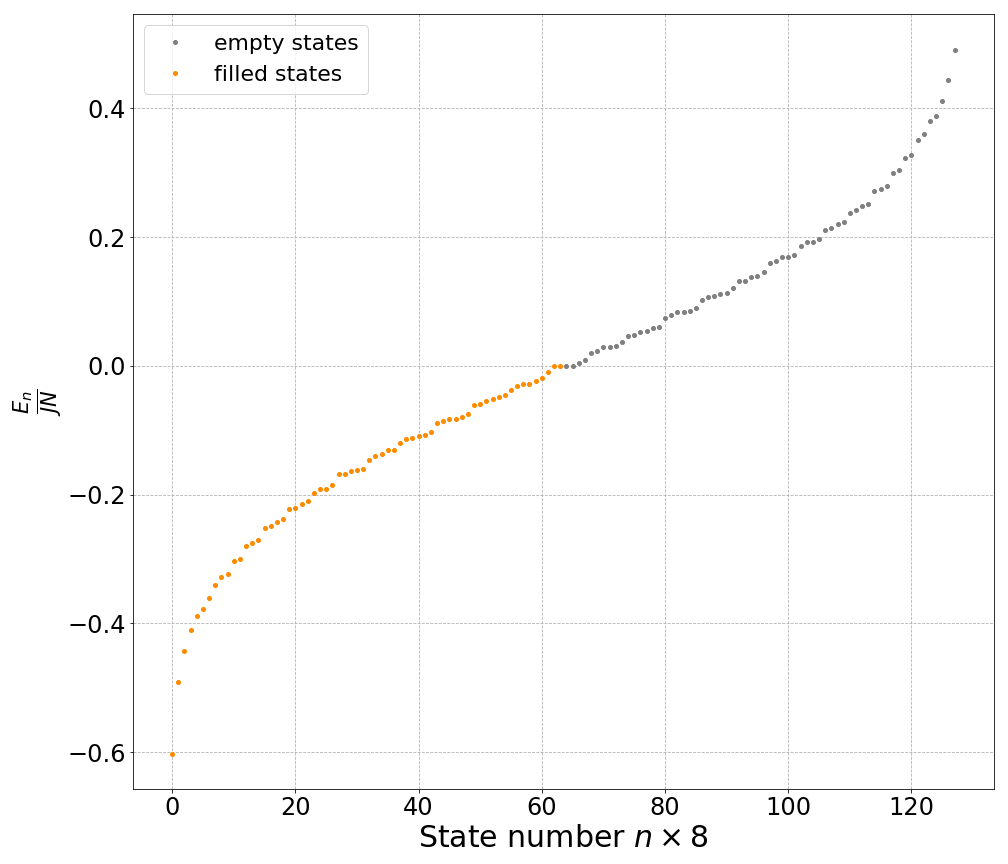
\includegraphics[scale=0.18]{figures/FreeFullSpecBatch_m0_L10.png}
    \end{minipage}%
    \begin{minipage}{0.5\textwidth}
    \centering(B)
    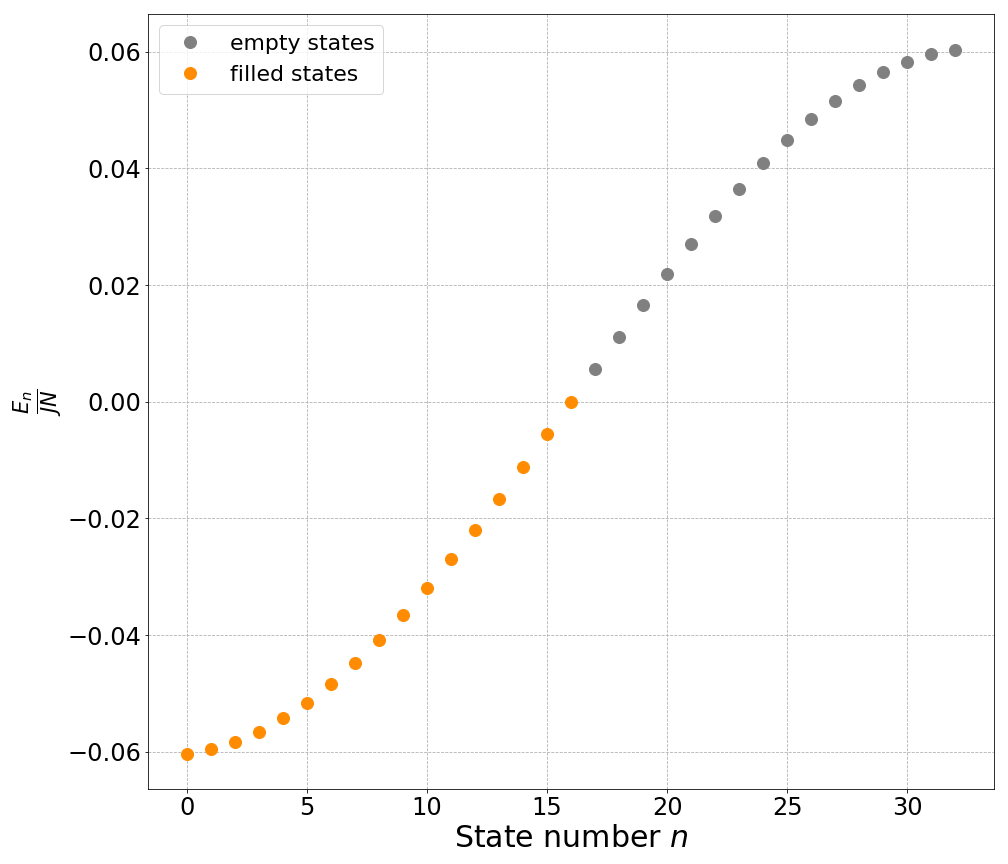
\includegraphics[scale=0.182]{figures/FreeFullSpecBatch_m0_L33.png}
    \end{minipage}
     \caption{Full spectrum of the Hamiltonian in real space. (A) Spectrum for $N=14$ taking batches of 8 eigenvalues to show the spectrum structure and avoid clutter. (B) Single particle excitation spectrum for $N=33$.}
    \label{fig:masslesFullSpecB}
\end{figure}

In figure \ref{fig:masslesFullSpecB} the orange dots are the filled states of the Dirac sea with negative energy, while the gray ones correspond to empty states above the Fermi level with positive energy (cf. \ref{sec:XXmodel}). \\

Similarly, we can plot the single particle excitation spectrum for a longer chain shown in figure \ref{fig:masslesFullSpecB} (right panel). This is possible as the system is non-interacting and the many-body wave function factorizes in a product of single-particle states. This decomposition has the advantage of avoiding the exponential scaling of the Hilbert space dimension by simulating the dynamics of a single particle. As we see the single-particle excitation spectrum is qualitatively very similar to the spectrum of the XX-model without a transverse field plotted in figure \ref{fig:XXSpec}.


\begin{figure}[htb]
    \centering
    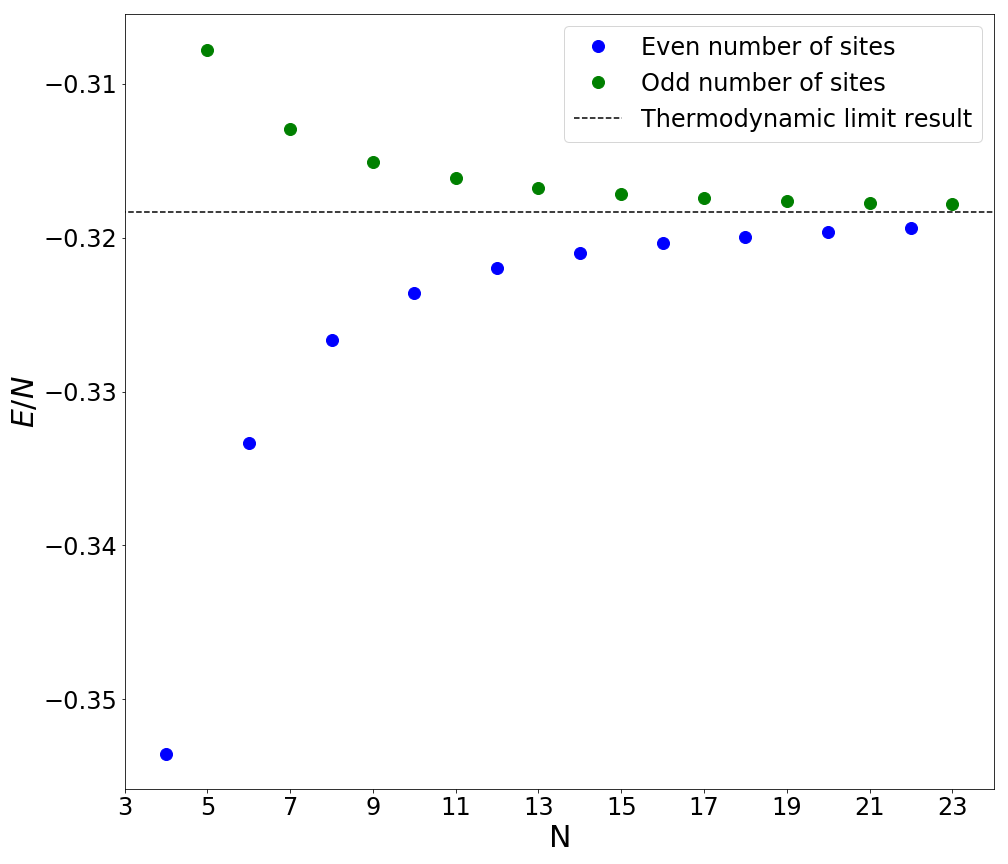
\includegraphics[scale=0.25]{figures/GroundStateE.png}
    \caption{Ground state energy per site for $N\in[4,24]$ for even and odd number of particles. The dashed black line is the result in the thermodynamic limit where $E_0/N=-1/\pi$}
    \label{fig:GSenergy}
\end{figure}


Moreover, we simulate the free Schwinger model from $N=4$ up to $N=24$ having as an objective to compute the smallest eigenvalue of the Hamiltonian, which corresponds to the ground state energy. Having the smallest eigenvalue we can compute the energy density for each lattice size, which we see from figure \ref{fig:GSenergy} approaches the thermodynamic limit value $-1/\pi$. Hence the free massless model corresponds with an XX spin chain without a transverse magnetic field. \\


\begin{figure}[htb]
    \begin{minipage}{.5\textwidth}
    \centering(A)
    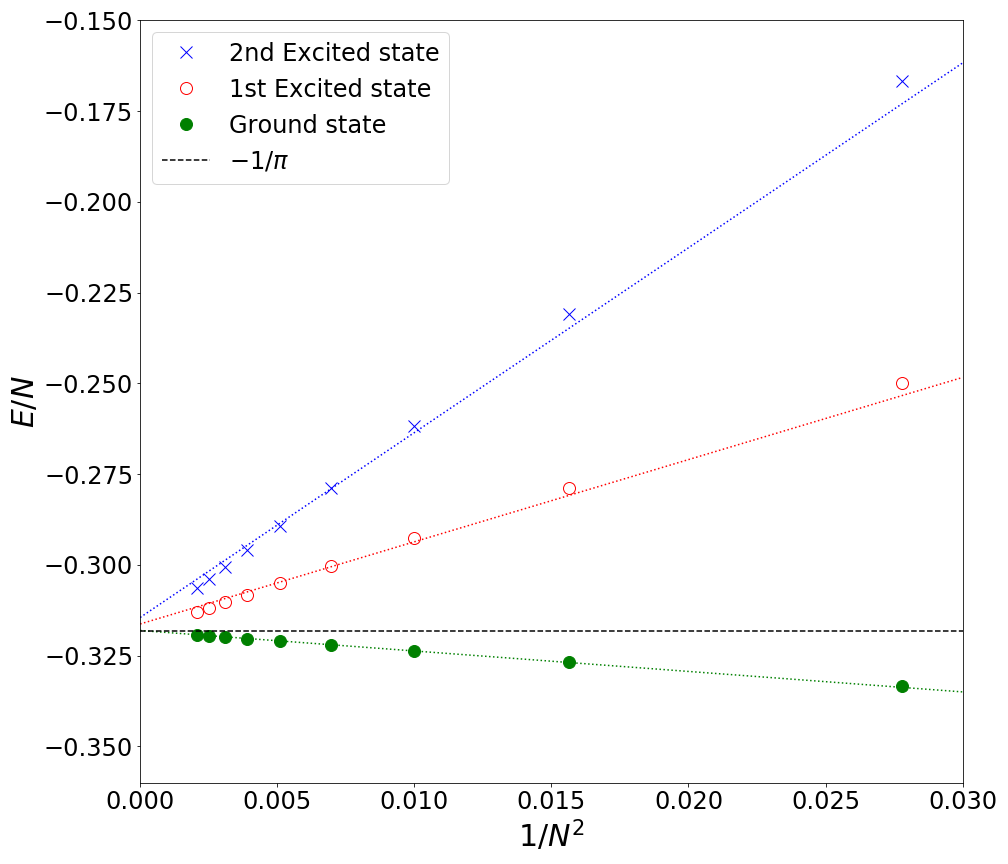
\includegraphics[scale=0.18]{figures/ExcitedStatesEven_m0_N-2.png}
    \end{minipage}%
    \begin{minipage}{0.5\textwidth}
    \centering(B)
    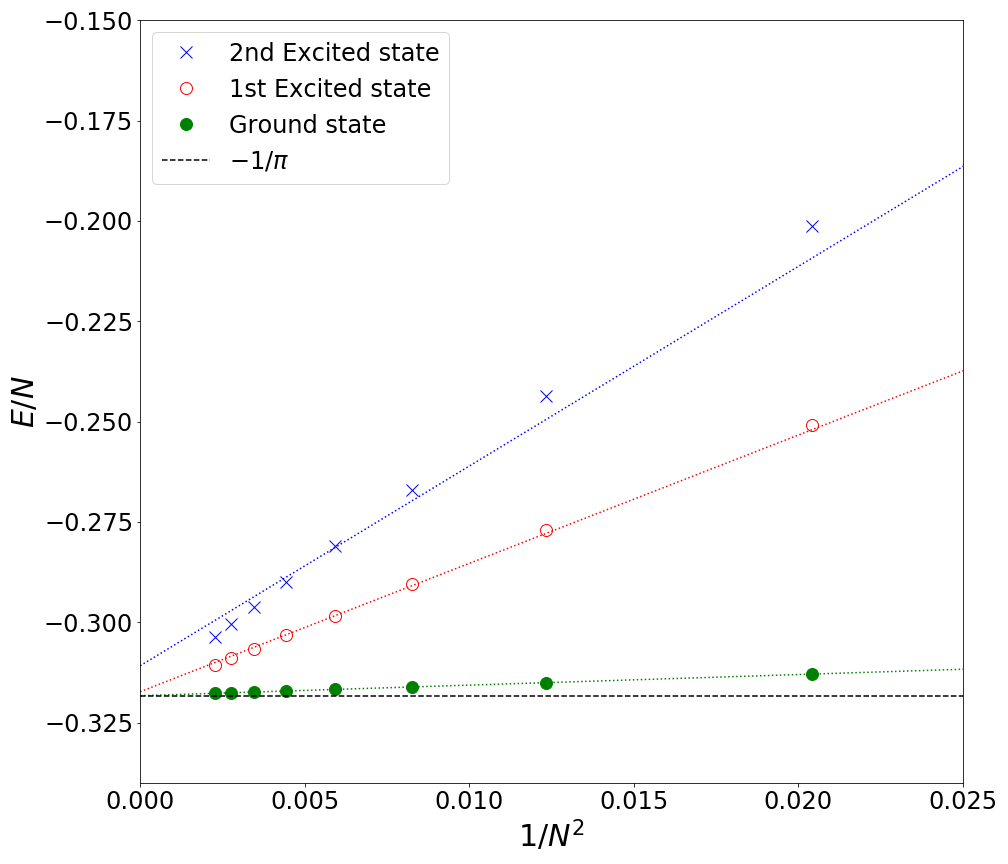
\includegraphics[scale=0.18]{figures/ExcitedStatesOdd_m0_N-2.png}
    \end{minipage}
    \caption{Plot of the ground state and the first two excited states energy densities versus the inverse of the number of sites squared with $N\in[4,22]$. Normalization of the energy density with $m$ is made to preserve the y scale. (A) Even number of particles. (B) Odd number of particles. A linear fit is made to determine numerically the ground state energy}\label{fig:excitedStatesMassles}
\end{figure}

Additionally, in figure \ref{fig:excitedStatesMassles} we show the energy densities of the first three excited states of the system for various lattice sizes. From the plots, we see how the all the states approach rapidly the thermodynamic energy density $-1/\pi\approx-0.318309$. To make this idea precise, note that the energy density for one dimensional free systems should scale roughly as the particle in a box energy density $$\frac{E_0}{N}\sim \frac{1}{N^2}.$$ 

Hence, if we plot the energy density of our model against $N^{-2}$ and make a linear fit to the simulation data, we can extract the value of the energy density in the thermodynamic limit. The linear fits are shown in \ref{fig:excitedStatesMassles}. It is also crucial to note, that from these plots we can infer that there is no energy gap between the ground state and the first excited states for the free massless lattice Schwinger model in the thermodynamic limit. This is clear as all the three linear fits are converging towards $-1/\pi$ in the limit of $N\to\infty$ in figure \ref{fig:excitedStatesMassles}. We can determine numerically the intercept of the best fit lines to extrapolate the thermodynamic value, doing this gives us the following results

\begin{equation}
\frac{E_0}{N} = -0.31797, \quad \text{N even };\quad \frac{E_0}{N} = -0.31832, \quad \text{N odd}.
\end{equation}


Thus, the numerical result extracted from our simulations is precise to within a part in one thousand compared to the thermodynamic limit energy density for the XX-model result, which is very very close. 



\section{The free massive Schwinger model}

The second model we will explore is the massive Schwinger model in absence of electromagnetic field but with non-zero mass, i.e. an XX-model with a traverse staggered magnetic filed. The Hamiltonian we will simulate is \ref{eq:XXHamilMass}. To obtain the energy levels and the spectrum of the Hamiltonian we use the exact diagonalization method in Quspin. First, we plot the full spectrum in real space for different mass values in figure \ref{fig:SpecMassive}. This is done to study how varying the fermion mass affects the eigenvalue structure. In figure \ref{fig:SpecMassive} the energy of each state $E_n$ is normalized with the mass in order to fix the $y$ scale of the plots.

\begin{figure}[htb]
	\begin{minipage}{.5\textwidth}
		\centering(A)
		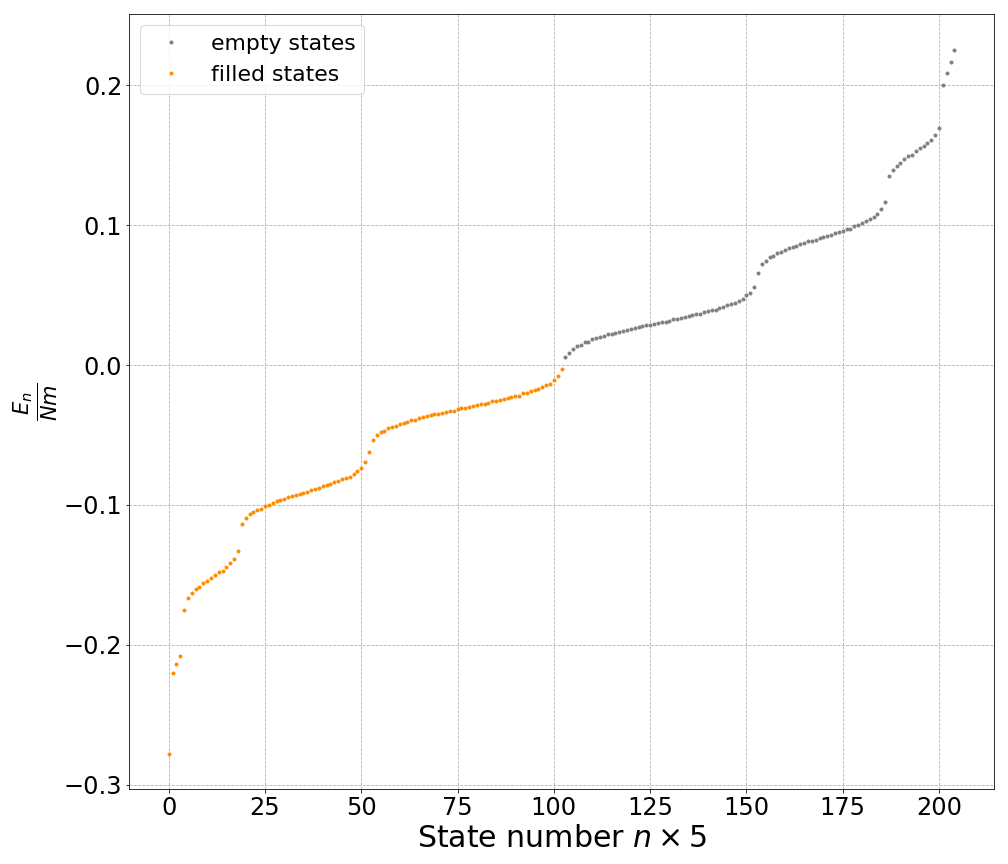
\includegraphics[scale=0.18]{figures/FreeFullSpec_m2.png}
	\end{minipage}%
	\begin{minipage}{0.5\textwidth}
		\centering(B)
		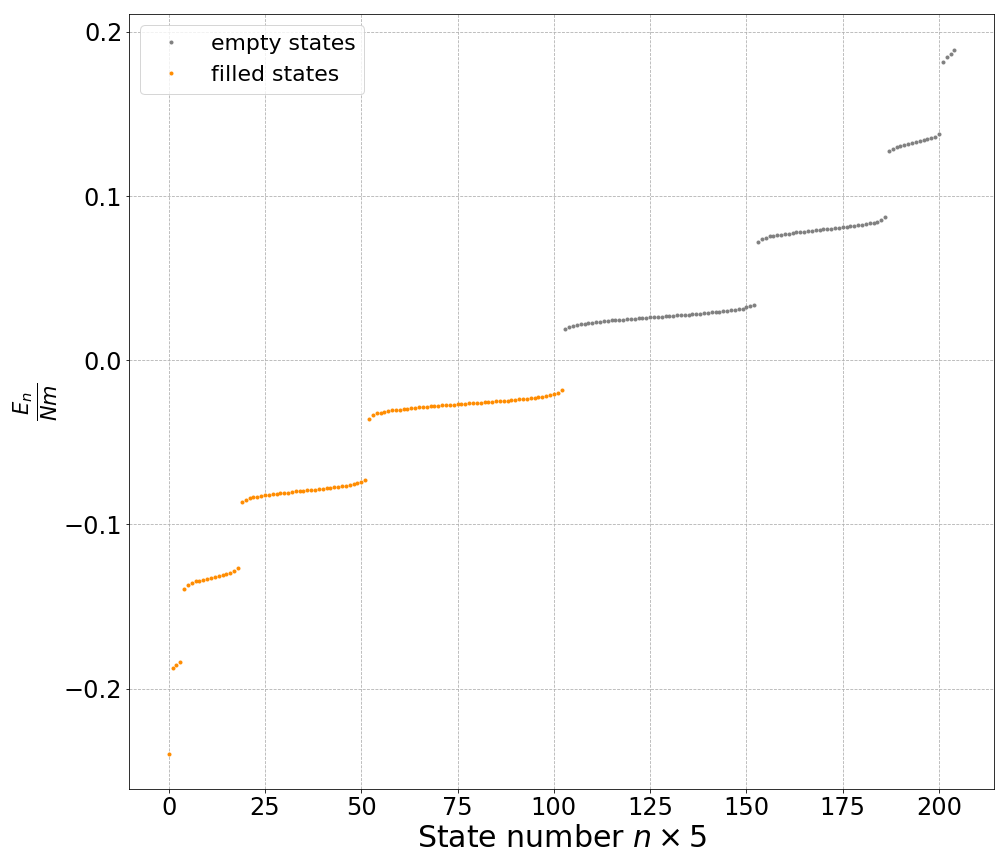
\includegraphics[scale=0.18]{figures/FreeFullSpec_m4.png}
	\end{minipage}
	\begin{minipage}{.5\textwidth}
		\centering(C)
		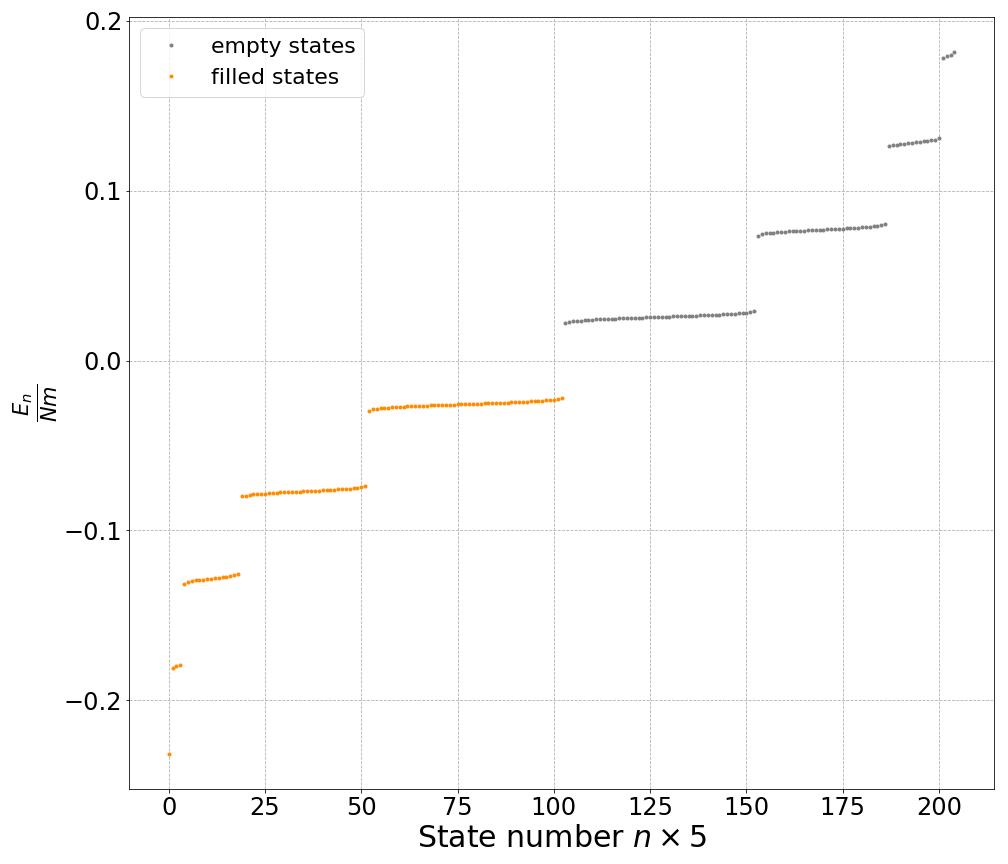
\includegraphics[scale=0.18]{figures/FreeFullSpec_m6.png}
	\end{minipage}%
	\begin{minipage}{0.5\textwidth}
		\centering(D)
		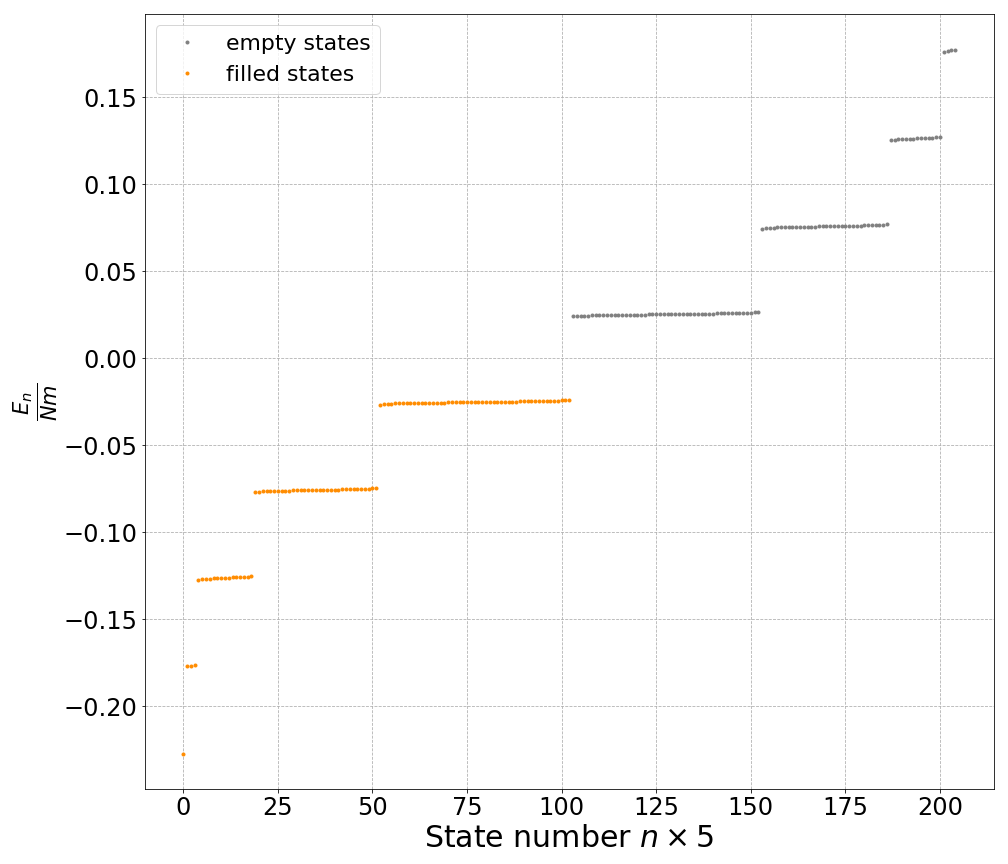
\includegraphics[scale=0.18]{figures/FreeFullSpec_m10.png}
	\end{minipage}
	\caption{Plot of the spectrum in real space for different values of the mass taking batches of 5 eigenvalues. (A) $m=2$, (B) $m=4$, (C) $m=6$ and (D) $m=10$.}\label{fig:SpecMassive}
\end{figure}


\begin{figure}
	\begin{minipage}{.5\textwidth}
		\centering(A)
		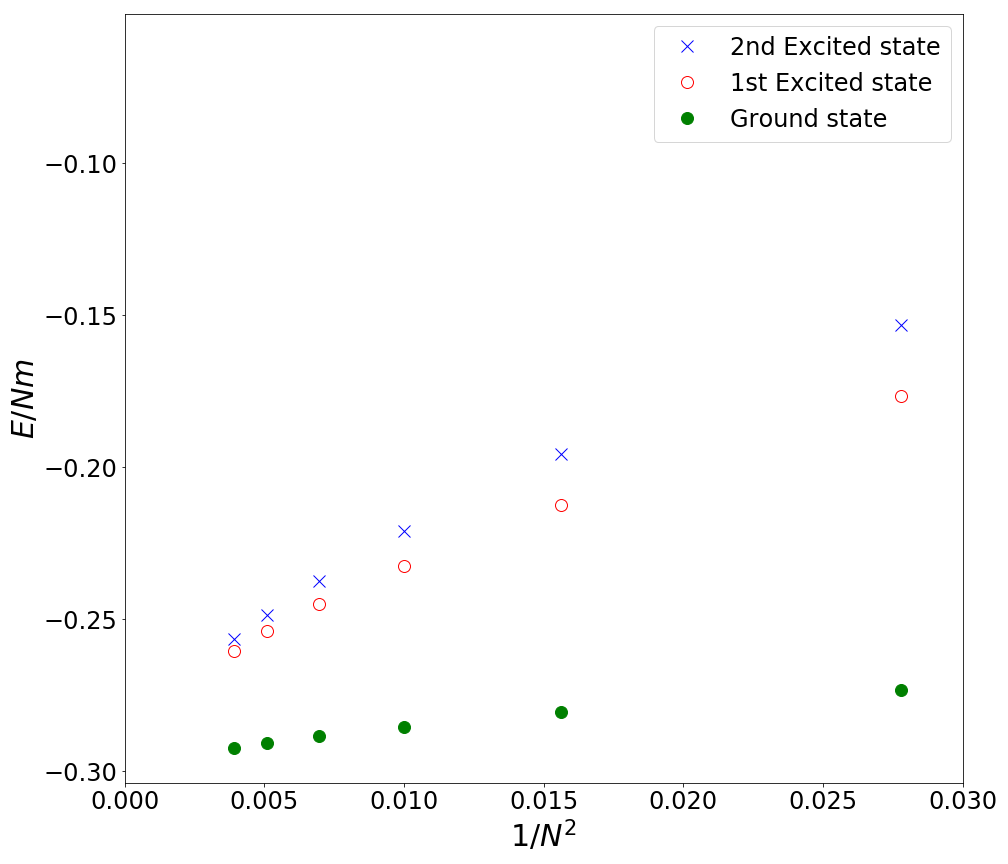
\includegraphics[scale=0.18]{figures/ExcitedStatesEven_m2_N-2.png}
	\end{minipage}%
	\begin{minipage}{0.5\textwidth}
		\centering(B)
		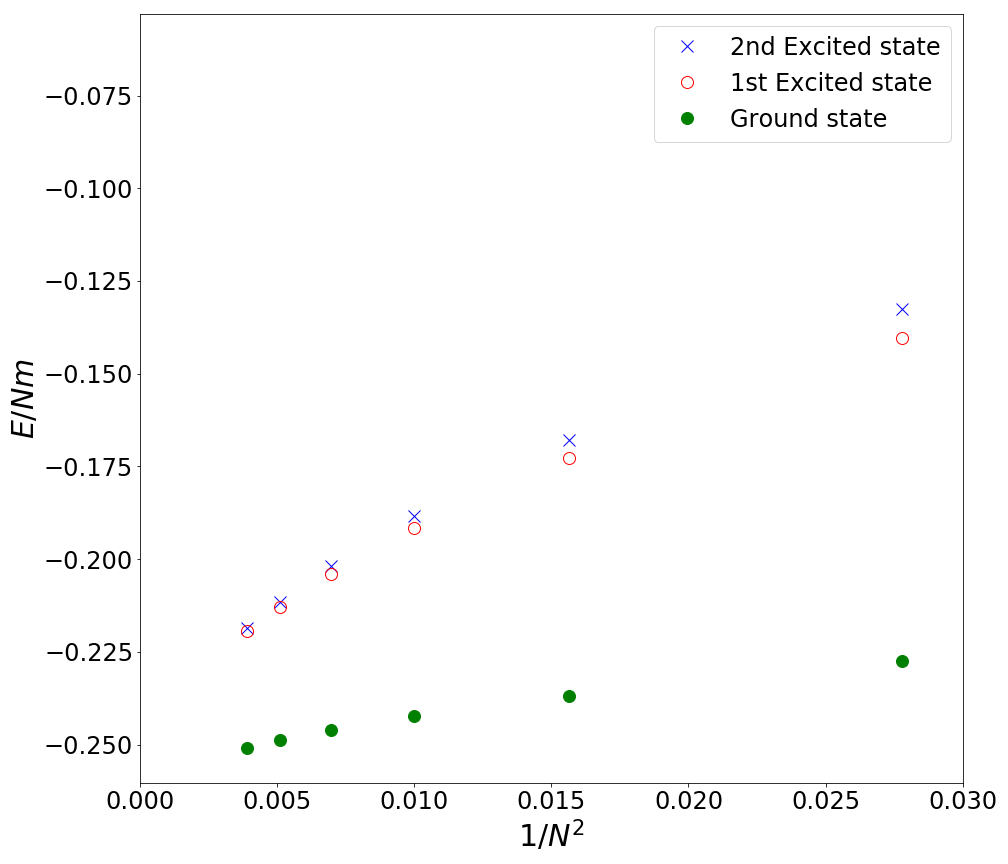
\includegraphics[scale=0.18]{figures/ExcitedStatesEven_m4_N-2.png}
	\end{minipage}
	\begin{minipage}{.5\textwidth}
		\centering(C)
		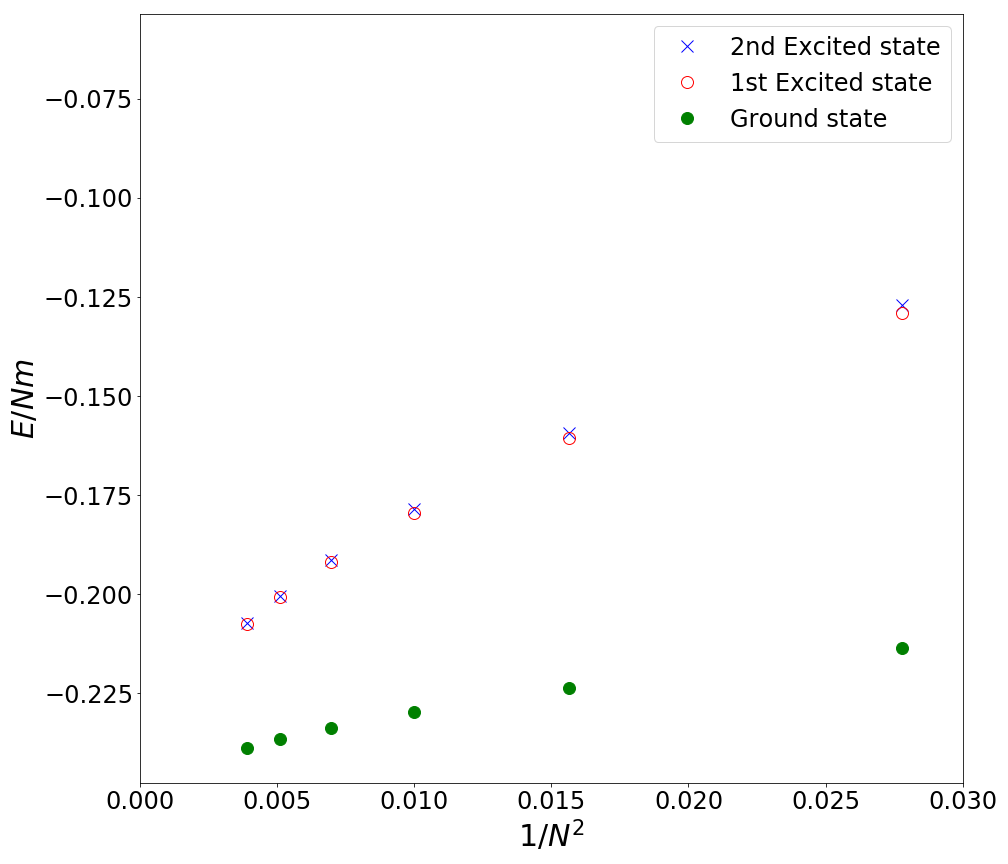
\includegraphics[scale=0.18]{figures/ExcitedStatesEven_m8_N-2.png}
	\end{minipage}%
	\begin{minipage}{0.5\textwidth}
		\centering(D)
		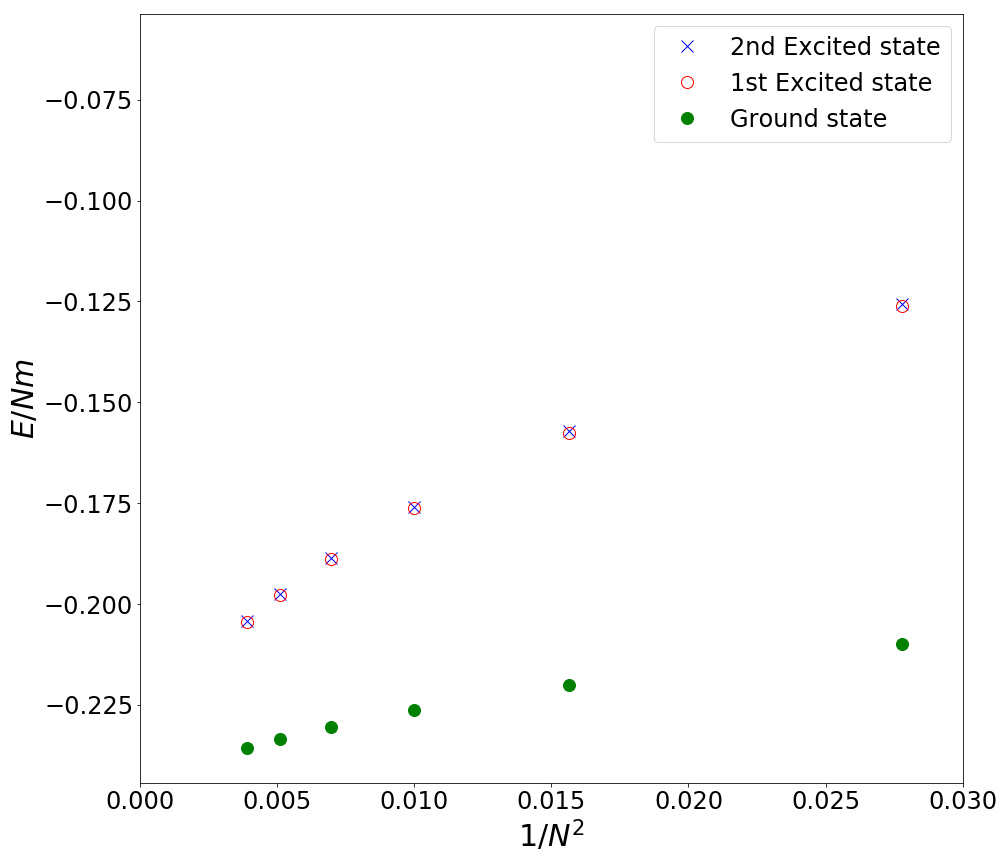
\includegraphics[scale=0.18]{figures/ExcitedStatesEven_m15_N-2.png}
	\end{minipage}
	\caption{Plot of the ground state and the first two excited states energy densities versus the inverse of the number of sites squared with $N\in[4,18]$ and $N$ even. Normalization of the energy density with $m$ is made to preserve the y scale. (A) $m=2$, (B) $m=4$, (C) $m=6$ and (D) $m=12$.}\label{fig:ExStMassive}
\end{figure}

A close examination of figure \ref{fig:SpecMassive} reveals a very interesting evolution of the spectrum with increasing mass. Note that as the mass parameter increases, the spectrum acquires a ladder-like structure, forming separate eigenvalue manifolds having roughly the same energy. Making the interpretation of this degeneracy rather simple, As the ratio $J/m$ decreases the Hamiltonian is dominated by a simple transverse field term (cf. \ref{sec:XYmodel}) 

\begin{equation}
H\sim \sum_n(-1)^n \sigma^z_n\label{eq:Zhamil},
\end{equation}


thus, in the limit of a very large mass, like the case of $m=10$ in figure \ref{fig:SpecMassive}, the Hamiltonian of the system is for all intents and purposes is \ref{eq:Zhamil}. Therefore, each separate manifold corresponds to a particular configuration of the spins (either aligned or anti-aligned with the $z$ axis) in the chain yielding a specific energy of this Hamiltonian. In particular, we observe that the single lowest energy state, i.e the ground state, is non-degenerate which means there exists a single spin configuration which minimizes the energy. This state corresponds to all the spin located on even sites being in $\ket{\downarrow}$ state, while the spins on odd lattice sites being in $\ket{\uparrow}$ state. A similar analysis can be made for the most energetic state, where all the spin located on odd sites are in the $\ket{\downarrow}$ state, while the spins on even lattice sites are in  the $\ket{\uparrow}$ state . As to the degenerate eigenvalue manifolds in the spectrum, they can be understood as follows,  several spin configuration yield the same energy, since permuting spins in different sites with the same configuration does not affect the valu of the energy. This fact accounts for the ladder-like structure of the spectrum, i.e this manifolds are invariant under a fixed number of permutations of the spins with the same state with respect to \eqref{eq:Zhamil}. This degeneracy is exact in the limit of very large mass $m\to\infty$, where the particle-antiparticle term of the Hamiltonian can be disregarded. Nevertheless, even though the effect of this term in small whenever $J/m<0.2$ it is not negligible as it "bends" the ends of each of the eigenvalue manifolds towards the closest manifold. Note that this bending effect is clear from the evolution of the spectrum as the mass parameter decreases. In the top left panel of figure \ref{fig:SpecMassive}, we see how the manifolds start to form and "rotate", separating from each other. In the top right panel, we can clearly differentiate each manifold, but we note that they are not fully degenerate in energy due to the particle-antiparticle term of the Hamiltonian. However, when the mass term becomes relevant compared to the value of $J$, as we see in the lower panel, the manifolds separate sharply and become increasingly degenerate.\\


Of particular interest to us is the structure of the ground state and the first excited states of the system, especially whether there exists of an energy gap between the ground state and the first excited state. To this end, we show in figure \ref{fig:ExStMassive} a plot of the energy density as a function of the inverse of the number of sites squared for an even number of sites taking different fermion massess \footnote{The plots for odd number of sites show essentially the same behavior and thus are not particularly more illuminating.}. \\

From figure \ref{fig:ExStMassive} we can conclude two important facts, First and foremost, there is an appreciable energy gap, $\Delta_E$, present as the first excited state energy density, plotted as a hollow red circles in figure \ref{fig:ExStMassive}, in the limit $n\to\infty$ clearly will not converge to the ground state energy density, shown as filled green circles. Secondly, as the ratio $J/m$ decreases the appearance of the eigenvalue manifold degeneration becomes evident even for the first and second excited states. Namely, as the mass parameter increases as we see in \ref{fig:ExStMassive} (C) and (D) the first and second excited states overlap, effectively demonstrating the ladder-like structure of the spectrum which is becoming increasingly degenerate as mass increases.\\


Finally, let us comment on the appearance of the energy gap in the massive model. Analytically, we can define the energy gap for the single particle spectrum of the XX-model (cf. section \ref{sec:XXmodel}) as

\begin{figure}
	\centering
	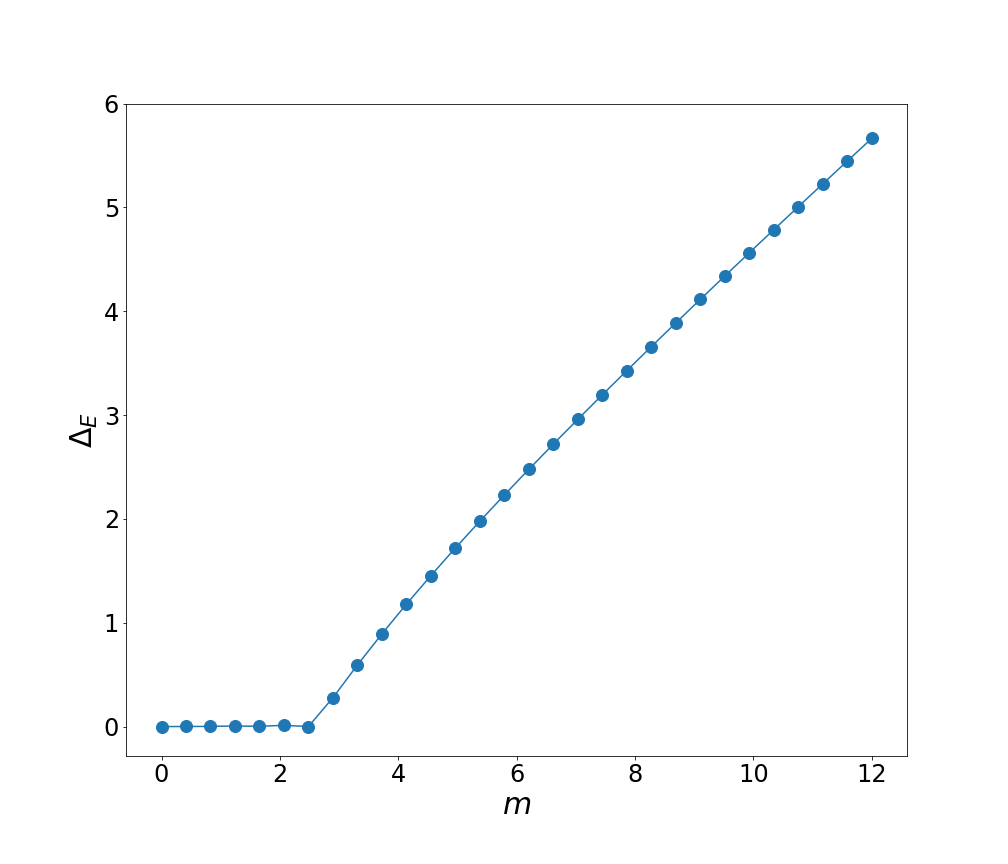
\includegraphics[scale=0.25]{figures/gap.png}
	\caption{Spectrum gap energy as a function of mass}
	\label{fig:gap}
\end{figure}

\begin{equation}
	   \Delta_E \overset{.}{=} \epsilon_{k=0} = (g - J).
\end{equation}
 
 Recall	 that in the case of the free massive lattice Schwinger model, $m/2$ is equivalent to the staggered transverse magnetic field $g$ in the XX-model (cf. section \ref{sec:latticeFormulation}). To make this precise, note that the energy gap should be linear on the mass and it should be shifted from zero by an amount $J$. In figure \ref{fig:gap} we show a plot of the energy gap resulting from simulations of systems with varying masses in the range $m\in [0,12]$. We see from this figure what we anticipated previously from studying the XX-model. The energy gap is indeed linear in mass and is shifted from zero by $J$ as expected. This confirms the equivalence between the free massive Schwinger model and the XX-model in the presence of a transverse staggered magnetic field.



\section{The interacting Schwinger Model}

Finally, the third model we will explore is the fully interacting Schwinger model (either massless or with non-zero mass). As a first simulation, we are interested in studying the energy density of the ground state for the massless interacting model. To do this we simulate the model varying the fermion charge $q_e$. We expect that whenever $q_e$ approaches zero the energy density of the ground state tends to $-1/\pi$ as the model becomes free.\\ 

\begin{figure}[h]
	\centering
	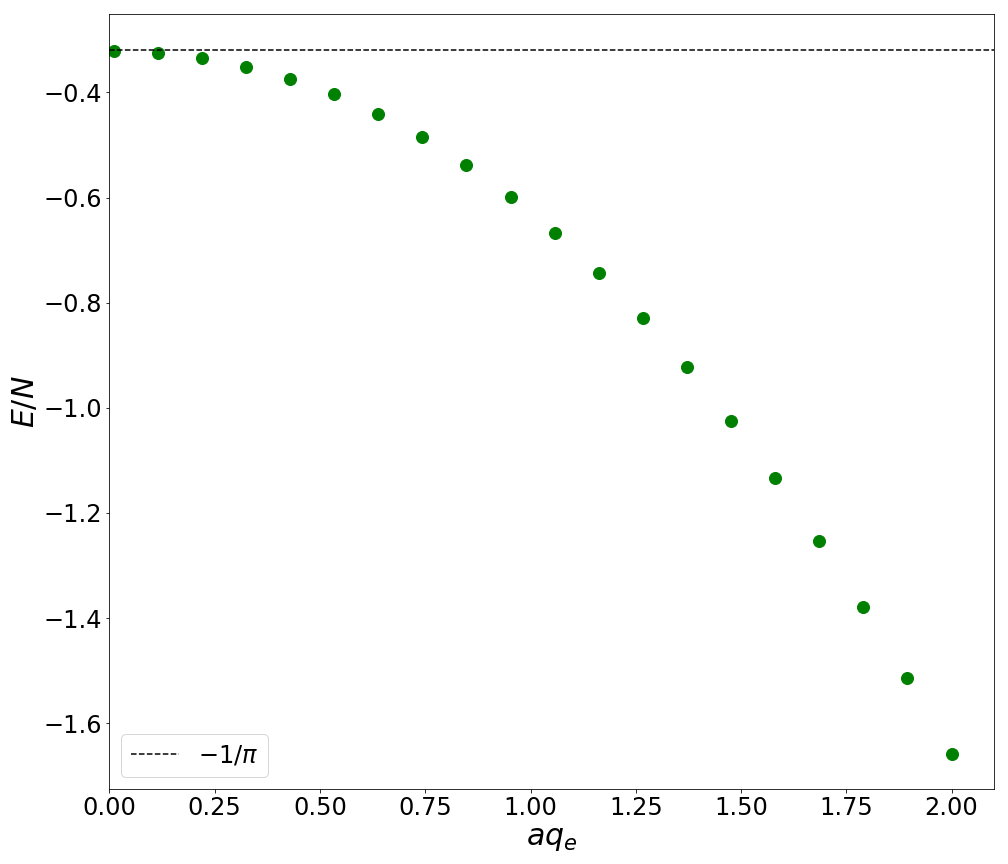
\includegraphics[scale=0.25]{figures/InteractingGsMassless}
	\caption{Plot of the ground state energy density for the massless interacting Schwinger model.}
	\label{fig:interactinggsmassless}
\end{figure}
Results of this simulation are shown in figure \ref{fig:interactinggsmassless}. We see that whenever the electron charge tends to zero the value of the energy density tends to the value of the free model as we should expect. Additionally, we see that for increasing values of $q_e$ the ground state energy per spin increases as the Hamiltonian is dominated by the electromagnetic energy stored in the electric field.\\

Additionally, beyond the ground state, we are interested in studying the behavior of the order parameters of the system. These parameters are the density of chiral condensate $\Gamma$ and the axial fermion density $\Lambda$. We have simulated a system of $N=14$ spins for $m\in\{0.0,2.0\}.$ and different values of the background electric field $\mathcal{E}_0$. Let us discuss briefly the results for each order parameter separately.\\

\begin{figure}[h]
	\begin{minipage}{.5\textwidth}
		\centering(A)
		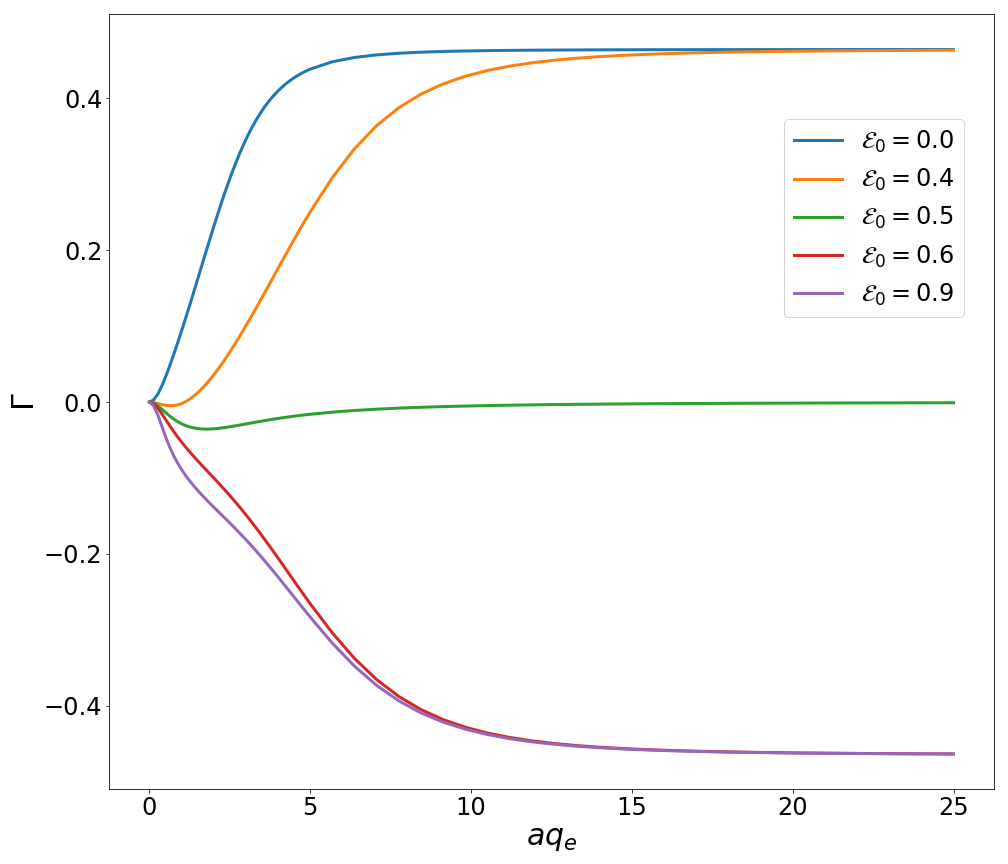
\includegraphics[scale=0.18]{figures/ChiralCond_m=00.png}
	\end{minipage}%
	\begin{minipage}{0.5\textwidth}
		\centering(B)
		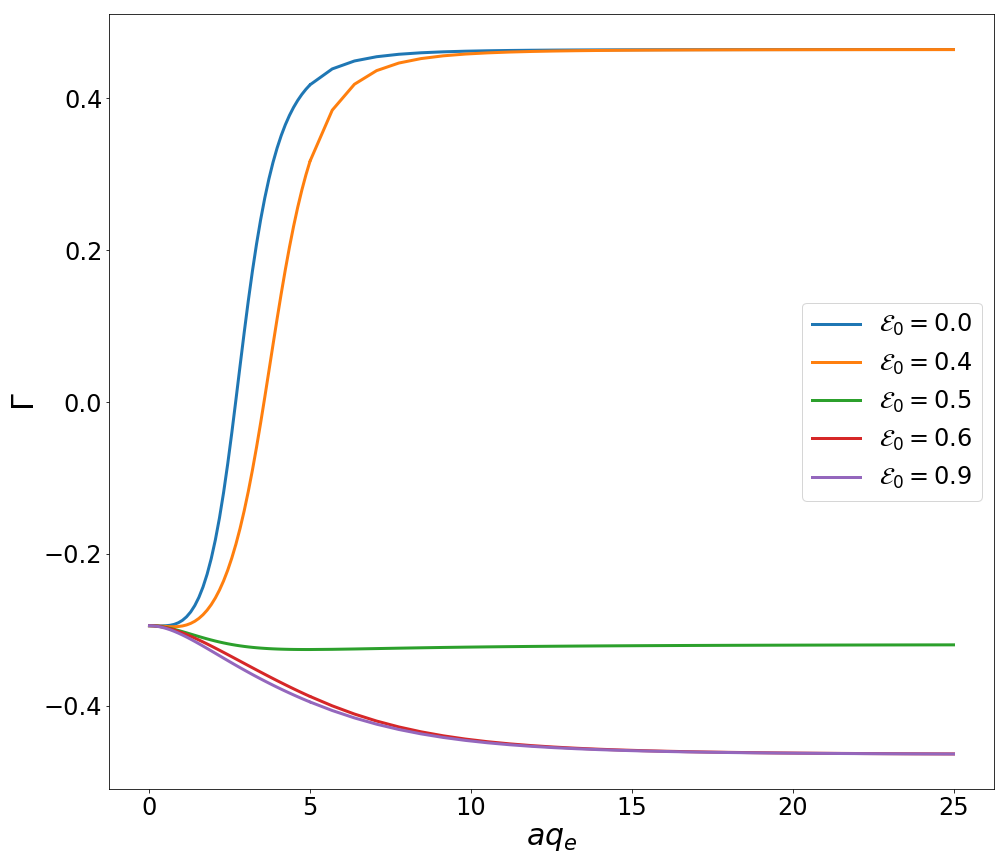
\includegraphics[scale=0.18]{figures/ChiralCond_m=20.png}
	\end{minipage}
	\caption{Plot of the density of chiral condensate as a function of $q_e$, $q_e\in[0,25]$. (A) Massless case $m=0$. (B) Massive Case $m=2.0$.}\label{fig:chiralcondq}
\end{figure}

First, in figure \ref{fig:chiralcondq} we observe the results of chiral condensate density of simulating systems with varying fermion charge. Note that we have selected values greater and smaller than the critical value of $\mathcal{E}_0=0.5$ where the phase transition occurs. Additionally observe that the value $\mathcal{E}_0=0.5$ sharply separates the regions $\mathcal{E}_0>0.5$ and $\mathcal{E}_0<0.5$. We see that in both this regions as fermion charge increases the values of $\Gamma$ approach the approximate values $\Gamma \approx \pm 0.45 $. This means that there are two distinct field configurations separated by $\mathcal{E}_0=0.5$. Recall, that in the first chapter we have discussed how the energetics of pair production in one-dimensional space gives rise to this critical behavior (cf section \ref{ssec:BackgroundField}). The appearance of two separate regions we observe in figure \ref{fig:chiralcondq} is a reflection of the dynamics a particle-antiparticle production due to the background field. Finally, note that the behavior for the massive case roughly the same as the massless one. The only difference is that whenever $q_e\to0$ in the massive case, $\Gamma\neq0$. Therefore, we can conclude that the presence of mass fixes a non-zero value of the chiral condensate. This can be understood by noting that the mass Hamiltonian 

\begin{equation*}
	H_{\text{mass}}\sim \sum \sigma^z,
\end{equation*}

being proportional to $\sigma^z$ is clearly relevant for the value of $\Gamma$ (cf. section \ref{sec:latticeFormulation}). However, the reader might ask what about the effective mass terms introduced the presence: of the electric field? Don't they also contribute to $\Gamma$? The answers to these questions are straightforward. Note that from the plots of the effective mass coupling (cf. figures \ref{fig:effMassE} and \ref{fig:effMassXi}) we can see their relative strength is basically equal, however, they appear in the Hamiltonian with opposite signs therefore, their contributions to $\Gamma$ gets canceled and the net effect is rather small.\\

\begin{figure}[h]
	\begin{minipage}{.5\textwidth}
		\centering(A)
		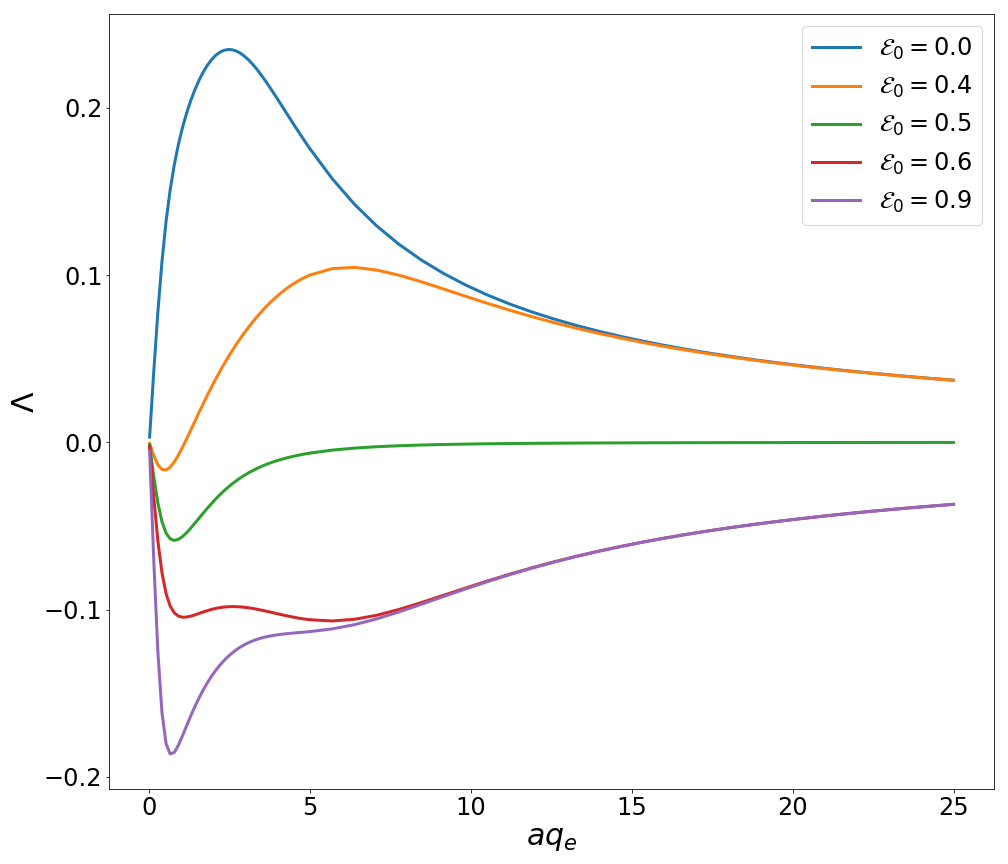
\includegraphics[scale=0.18]{figures/axial_m=00.png}
	\end{minipage}%
	\begin{minipage}{0.5\textwidth}
		\centering(B)
		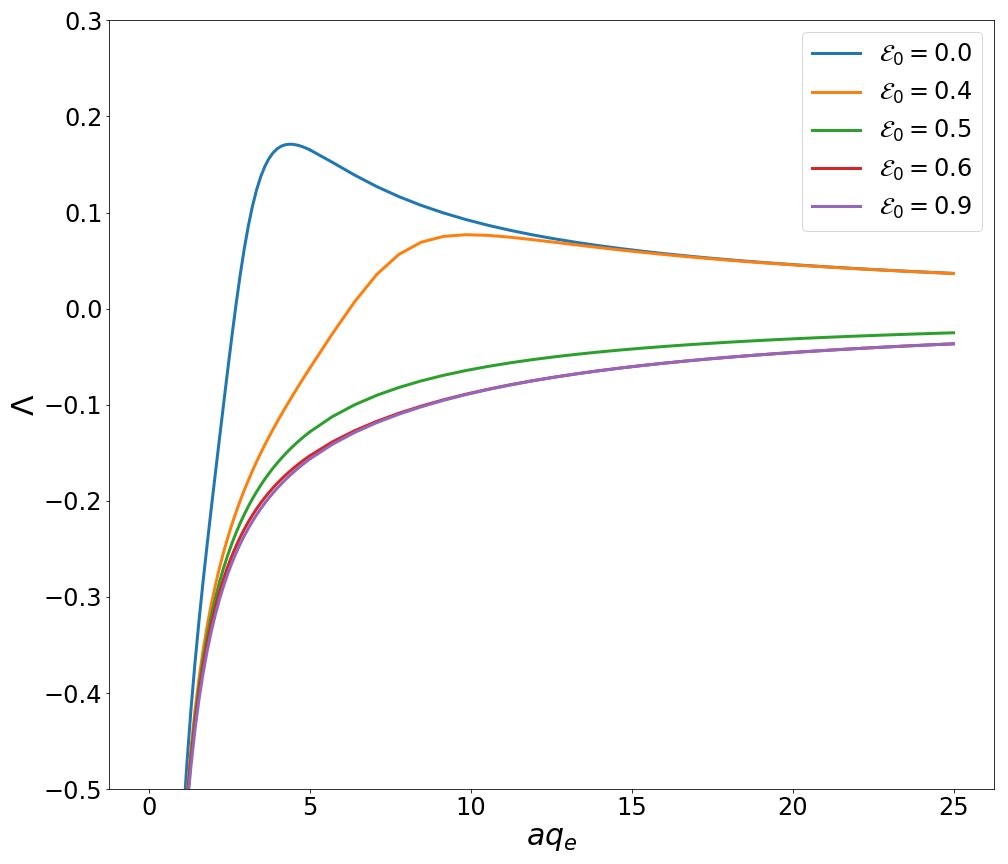
\includegraphics[scale=0.18]{figures/axial_m=20.png}
	\end{minipage}
	\caption{Plot of the axial fermion density as a function of $q_e$, $q_e\in[0,25]$ for different background field values. (A) Massless case $m=0$. (B) Massive Case $m=2.0$.}\label{fig:axialdensityq}
\end{figure}

Second, in figure \ref{fig:axialdensityq} we observe the results from the axial fermion density obtained by simulating systems with varying fermion charge. We see that in the case $m=0.0$, there is a behavior similar to the one described for the density of chiral condensate. There are two distinct values where the curves for $\Lambda$ overlap as $q_e$ increases. Nevertheless, the plot for $m=2.0$ shows a very different result. In this case, we see that the curves for $\Lambda$ for all values of $\mathcal{E}_0$ overlap and very rapidly tend towards zero. This can be understood by noting that $\Lambda$ is essentially the particle-antiparticle portion of the Hamiltonian (cf. section \ref{sec:latticeFormulation}) and thus as the background field increases the phenomenon of pair production begins in the system in order to screen the background field. However, as soon as massive particle-antiparticle pairs are created from vacuum dielectric breakdown, the expectation value of the axial fermion density tends to vanish. Nevertheless, as opposed to the massless case, in the massive case the production of a particle anti-particle pair from vacuum costs at least twice the rest mass of the particle. Therefore, these pairs are rapidly created to screen the background field until it is no longer energetically favorable for the vacuum to create any more pairs and the axial density rapidly vanishes.\\

Moreover, the relationship between $\Gamma$ and $\Lambda$ with mass was studied for $\mathcal{E}_0=0.0,\,0.5,\,0.9$ and $m\in[0,1]$. The results are shown in figure \ref{fig:axialchiralmass}. We can see from the plots that for increasing $m$ both $\Lambda$ and $\Gamma$ curves overlap and tend to a fixed value. In the case of $\Lambda$, we see a steady decrease towards $0$ which means that the axial fermion density vanishes for $m\neq0$. This is consistent with was commented before in reference to figure \ref{fig:axialdensityq}.\\

\begin{figure}[h]
	\begin{minipage}{.5\textwidth}
		\centering(A)
		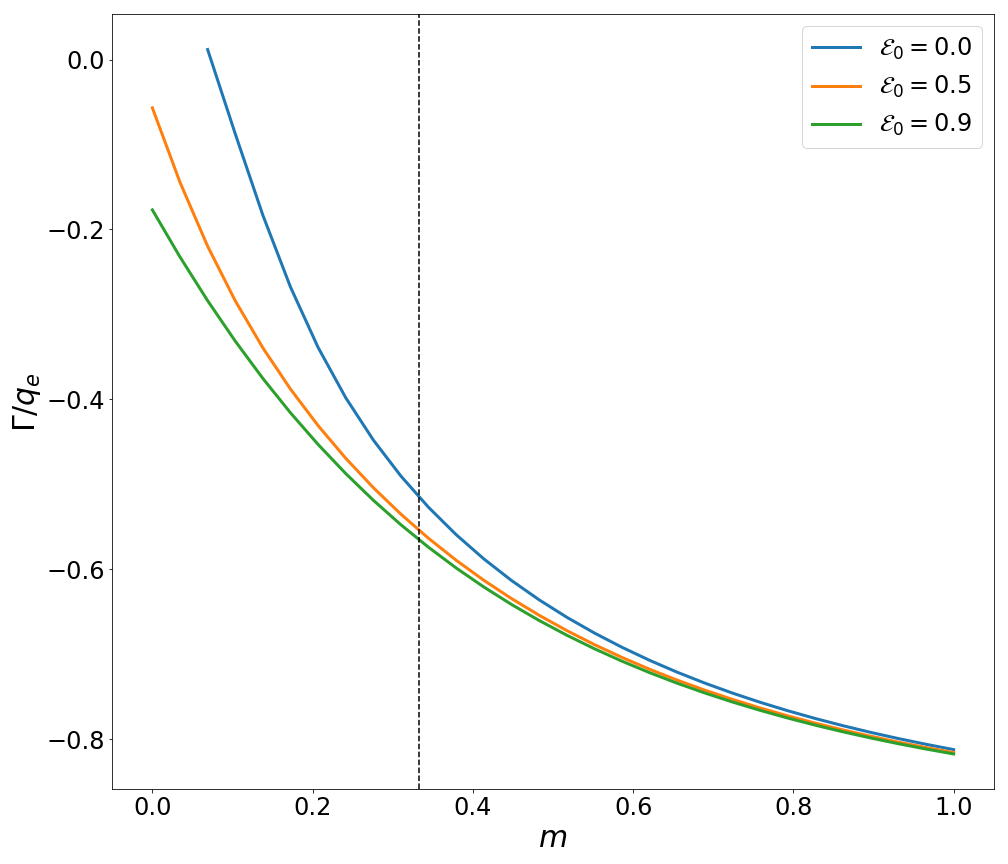
\includegraphics[scale=0.18]{figures/ChiralCond-mm.png}
	\end{minipage}%
	\begin{minipage}{0.5\textwidth}
		\centering(B)
		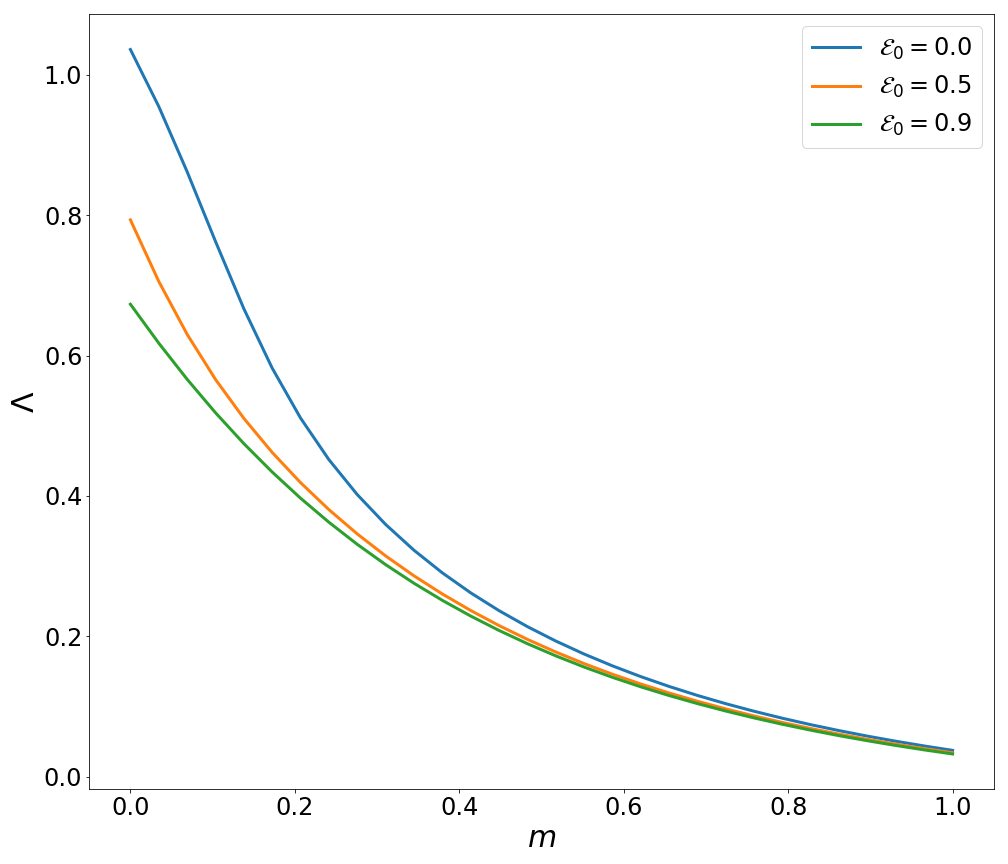
\includegraphics[scale=0.18]{figures/AxialDensity-mm.png}
	\end{minipage}
	\caption{Plot of the order parameters as a function of fermion mass $m\in[0,1]$ for different background field values.The fermion charge $q_e$ is set to $1$. (A) $\Gamma/q_e$ as a function of $m$. Dotted line at $m/g=0.3$ for reference. (B) $\Lambda$ as a function of $m$.}\label{fig:axialchiralmass}
\end{figure}

Additionally, we can say qualitatively that from the form of $\Gamma$ at $\mathcal{E}_0$ there is a phase transition at a value close to $m/q_e = 0.3$.  Above $\mathcal{E}_0=0.5$ the chiral symmetry of the theory is broken due to the background field and there are two degenerate vacuum states \cite{Coleman1976,Hamer1997}. Note the different behavior for $\mathcal{E}_0=0.0$ and for $\mathcal{E}_0=0.9$, where roughly at $m/q_e = 0.3$ the curves diverge approaching $\Gamma/q_e \approx \pm 0.2$ at vanishing mass.

\section{Quantum quenches in the Schwinger model}

The study of closed quantum systems out of equilibrium is of the utmost importance in order to understand the dynamics of nature out of the equilibrium regime. Non-equilibrium processes are readily present in most areas of physics, therefore, a better understanding of non-equilibrium phenomena is paramount to a broader understanding of nature and its nuances. Nonetheless, such ventures out of equilibrium are in general very hard problems to tackle, and solutions are often absent. The question is then: how can we study the out of equilibrium dynamics of quantum systems in a way that gives illustrative answers?\\

\begin{figure}[h]
	\centering
	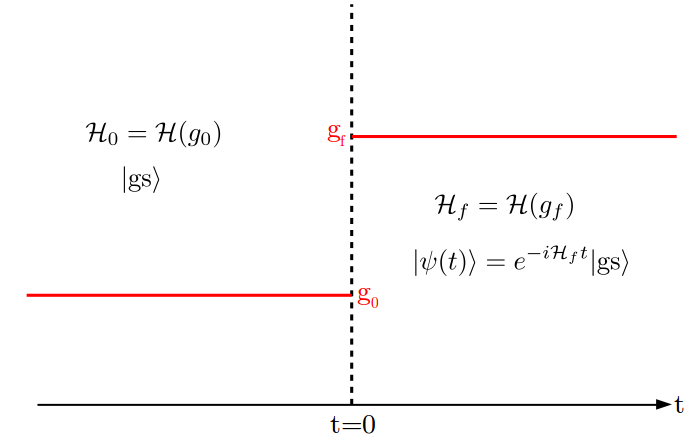
\includegraphics[scale=0.35]{figures/quenchProt}
	\caption{Quantum quench protocol.}
	\label{fig:quenchprot}
\end{figure}


There is a very large number of ways of driving quantum systems out of equilibrium, and most of them turn the exact calculation of system dynamics into a formidable and often impossible task. Therefore, the name of the game is to find a way to ``kick" the system out of equilibrium in a way that enables calculation of the most relevant system properties. One of the most popular ways to ``kick" a system out of equilibrium is known as a \emph{quantum quench} . The idea behind a quantum quench is to prepare the system in a non-equilibrium state whose evolution is dictated in terms of the system's Hamiltonian. This implies in particular, preparing the system in the ground state $\ket{\textrm{GS}}$ of a Hamiltonian $H_0$ and subsequently, evolving the state unitarily according to a different Hamiltonian $H_1$ 

\begin{equation*}
	\ket{\psi(t)} = e^{-i t H_1} \ket{\textrm{GS}};\quad t>0, \quad \comm{H_0}{H_1}\neq 0
\end{equation*}

Hereafter, let $H(g)$ be the system Hamiltonian dependent on some external parameter $g$, that can be, for example, an electric or magnetic field or the interaction strength between particles. In a \emph{global quantum quench} $H_0 = H(g_0)$ at some given initial value of the external parameter and at a fixed time, say $t=0$ a sudden switch in the Hamiltonian parameters occurs, $H_1=H(g_f)$ where $g_f$ is a new value of the parameter. Thus, the quenching protocol of interest to us consists of changes in Hamiltonian parameters of a given system (see figure \ref{fig:quenchprot}). There are also other popular quenching protocols: \emph{local quenches} where the quench is limited to a bounded regions of the system; \emph{sweeps} where the change in parameter has an explicit time dependence given some detailed protocol; and \emph{geometric quenches} where the spatial configuration of the system is changed, for example, a sudden change from periodic to open boundary conditions.

The objective of a quench is to study the evolution of observables that can give physical insight into the dynamics of the system, viz 

\begin{equation}
\expval{\mathcal{O}_1\cdot\mathcal{O}_2\cdot\ldots\cdot\mathcal{O}_n}(t) = \frac{\ev{\mathcal{O}_1\cdot\mathcal{O}_2\cdot\ldots\cdot\mathcal{O}_n}{\psi(t)}}{\ip{\psi(t)}}
\label{eq:expvalops}
\end{equation}

where each $\mathcal{O}_i$ is a local observable. Assuming that $H_1$ has a discrete spectrum $\{E_n\}$ and recalling that our time evolved state $ \psi(t)$ can be written in terms of our pre-quench ground state we can rewrite any expected value of a local operator $\mathcal{O}(t)$ as

\begin{equation}
\expval{\mathcal{O}}(t) = \sum_{m,n}\ip{\textrm{GS}}{E_m}\ip{E_n}{\textrm{GS}}\mel{E_m}{\mathcal{O}}{E_n}e^{-i (E_m-E_n)t}.
\label{eq:expvalobs1}
\end{equation}

Another important quantity in the study of quantum quenches is the Loschmidt amplitude

\begin{equation}
\mathcal{L}(t) = \ev{e^{iH_0 t}e^{-iH_f t}}{GS}=\ev{e^{-iH_f t}}{GS},
\end{equation}

since $\ket{GS}$ is the ground state of $H_0$ the last equality follows from the fact that $H_0\ket{GS}=0$. This amplitude quantifies how far from equilibrium a system is taken due to the evolution generated by Hamiltonian dynamics. Additionally, we can compute form the Loschmidt amplitude its modulus squared

\begin{equation}
L(t) = \abs{\mathcal{L}(t)}^2,
\end{equation}

known as the Loschmidt echo. This quantity gives a measure of the stability of the system dynamics along time evolution.\\

Thus, in a quantum quench one addresses several important aspects related to the dynamics of our system, namely:

\begin{itemize}
	\item \textbf{Thermodynamics:} Due to the sudden change in the systems Hamiltonian work is done to the system and its internal energy is abruptly altered. This sudden change generates a real-time evolution between equilibrium states of $H_0$ and $H_1$.
	\item \textbf{Real-time dynamics and relaxation:} As a consequence of the abrupt perturbation the system has to adjust and relax to an equilibrium state. The time scales and asymptotic behavior of such a process may give relevant physical information of our system.
	\item \textbf{Thermalization} Classically a system that is taken out equilibrium evolves to an equilibrium configuration after a sufficiently long time scale. On the context of quantum quench dynamics, an important question that has not been definitely answered is whether a closed quenched quantum system prepared in a non-equilibrium state can reach an equilibrium configuration without a coupling to an environment.
\end{itemize}

\subsection{Quenches from the free model}

The first type of quantum quench we will explore will be a quench starting from the free massless Schwinger model to the interacting massless Schwinger model. Therefore, for this particular quench, we take the initial Hamiltonian $H_0$ to be the Hamiltonian for the free massless model, i.e. the XX-model Hamiltonian with its corresponding ground state $\ket{GS}$.  The final Hamiltonians $H_f$, post quenching will be the Hamiltonian of the interacting massless Schwinger with background field for $\mathcal{E}_0=0.0$ and $\mathcal{E}_0=0.5$. For this quench, we will study two quantities that interesting in this context, First, we will study the Loschmidt echo density

\begin{equation}
\frac{|\mathcal{L}(t)|^2}{L} = \frac{L(t)}{L}.
\end{equation}

we call it a density as it is divided by the number of lattice sites. Second, we will study the expectation value of the density of chiral condensate between the ground state of the initial Hamiltonian and the time evolved state generated by the interacting Hamiltonian, viz

\begin{equation}
\tilde{\Gamma}(t)\overset{.}{=} \ev{\Gamma e^{-iH_f t}}{GS},
\end{equation}

and the same expectation value for the axial fermion density

\begin{equation}
\tilde{\Lambda}(t)\overset{.}{=} \ev{\Lambda e^{-iH_f t}}{GS}.
\end{equation}

Results for the Loschmidt echo density are shown in figure \ref{fig:loschmidtnoninteractingquenchmassless}.

\begin{figure}[h]
	\centering
	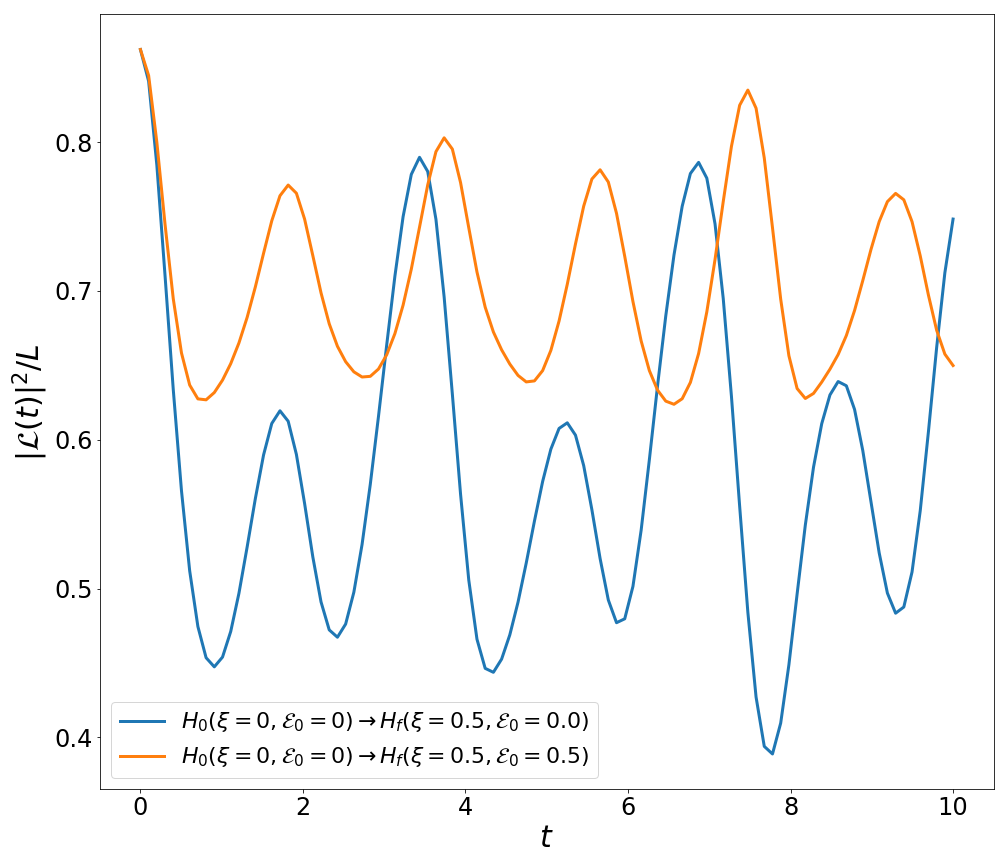
\includegraphics[scale=0.25]{figures/LoschmidtNonInteractingQuenchMassless}
	\caption{Plot of the Loschmidt echo density as a function of time for a quench from the free model to the interacting model. Blue line corresponds to $\mathcal{E}_0=0.0$ . Yellow line corresponds to $\mathcal{E}_0=0.5$.}
	\label{fig:loschmidtnoninteractingquenchmassless}
\end{figure}

In figure \ref{fig:loschmidtnoninteractingquenchmassless} we can see the oscillatory behavior of the Loschmidt for both values of the background field. Both plots have a similar oscillation frequency, however, see that clearly, the oscillation amplitude is greater for the quench to the interacting model with $\mathcal{E}_0=0.0$. \\


The results for the chiral condensate density are shown in figure \ref{fig:chiralnoninteractingquench}. In this plot, we see how the expectation value of $\Gamma$ oscillates in both cases with roughly the same frequency, but again as mentioned earlier, the plot for zero background field has a greater amplitude than the case of a non-zero background field. 

\begin{figure}[h]
	\centering
	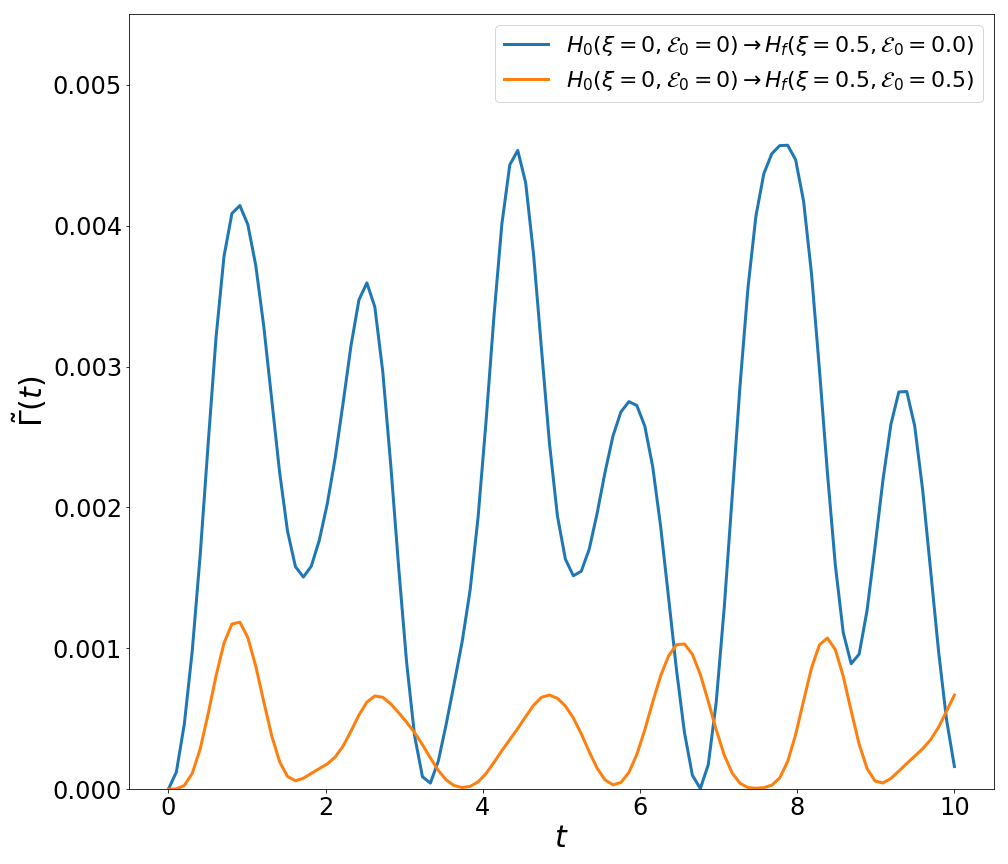
\includegraphics[scale=0.25]{figures/chiralNonInteractingQuenchMassless.png}
	\caption{Plot of the density of chiral condensate as a function of time for a quench from the free model to the interacting model. Blue line corresponds to $\mathcal{E}_0=0.0$ . Yellow line corresponds to $\mathcal{E}_0=0.5$.}
	\label{fig:chiralnoninteractingquench}
\end{figure}

\subsection{Quenches between background fields}

Finally, the second type of quantum quench we are interested in is one which the initial Hamiltonian is the massless interacting Hamiltonian without background electric field to the Hamiltonian corresponding to the massless interacting model with a background field $\mathcal{E}_0=0.5$. In figure \ref{fig:loschmidtinteractingquench} we can see how the Loschmidt echo density evolves with time. Note that, the time evolution is given by an oscillatory function resembling a cosine function. Hence, we can say that the dynamics of the interacting model is oscillatory whenever the background field changes abruptly. This makes sense if we note that if the background field is suddenly switched on it will induce dielectric breakdown from the vacuum followed shortly by pair production. This will screen the electric field effectively reducing its value below the critical one (cf. subsection \ref{ssec:BackgroundField}).

\begin{figure}[h]
	\centering
	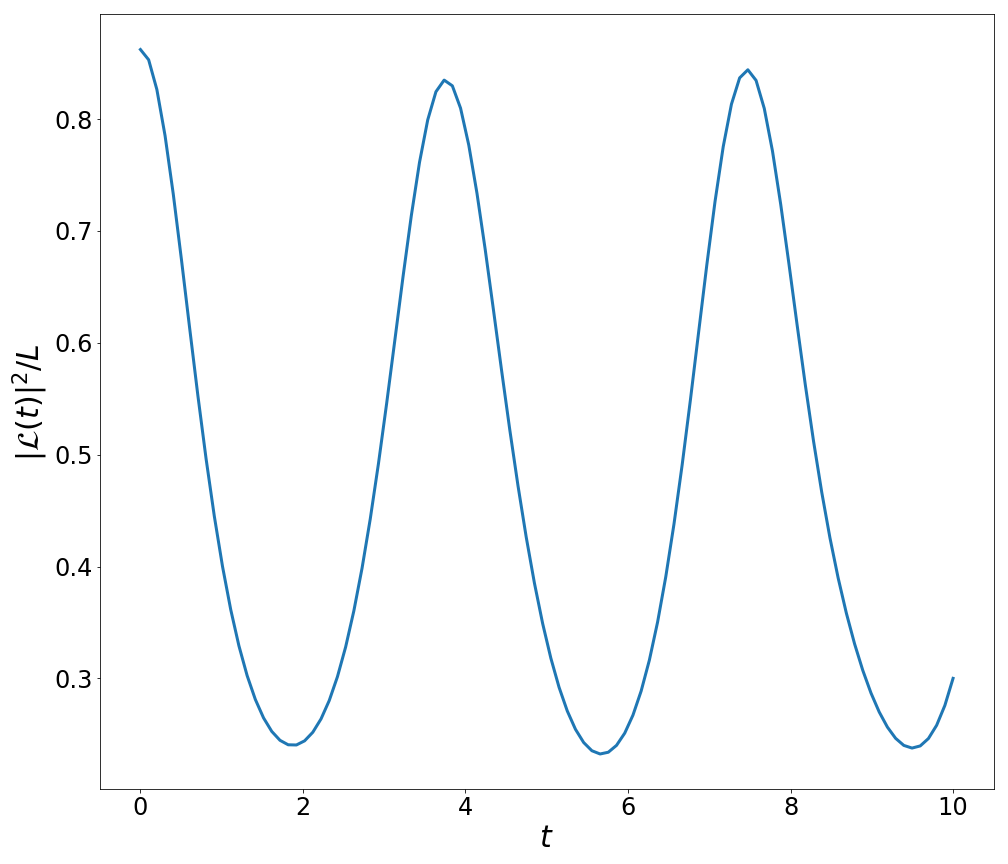
\includegraphics[scale=0.25]{figures/LoschmidtInteractingQuenchMassless.png}
	\caption{Plot of the Loschmidt echo density as a function of time  for a quantum quench between the massless interacting Hamiltonian with $\mathcal{E}_0=0.0$ to the massless interacting Hamiltonian with $\mathcal{E}_0=0.5$.}
	\label{fig:loschmidtinteractingquench}
\end{figure}

Finally, in figure \ref{fig:orderparamsquech} we see the time evolution of the two order parameters characterizing the critical behavior induced by the background filed. Note that both plots show an oscillating behavior which can be understood roughly in the same manner as we previously commented for the Loschmidt echo density. However, we see that the axial fermion density oscillates somewhat more randomly compared to the chiral condensate density. This can be traced back yet again, to the dynamics of pair-production induced by the background field, recall that the axial fermion density operator is essentially a particle-antiparticle creation-annihilation operator. Hence, it is very sensitive to the presence of particle-antiparticle pairs, and we expect it to oscillate more rapidly. Furthermore, observe that the dynamics of the density of chiral condensate are roughly the same as the ones we found from the quench between the free and interacting model. Nonetheless, the sharp oscillatory behavior of $\Gamma$ indicates to us that a quench from an eigenstate of the interacting model with $\mathcal{E}_0=0.0$ to an eigenstate of the interacting model with $\mathcal{E}_0=0.5$ is taking the system out of equilibrium. Moreover, besides taking the system out of equilibrium the quench is crossing a point where a phase transition occurs (cf subsection \ref{ssec:BackgroundField}) which fundamentally drives the system out of equilibrium and explains the abrupt changes and oscillatory behavior of the order parameters of the system.


\begin{figure}[h]
	\begin{minipage}{.5\textwidth}
		\centering(A)
		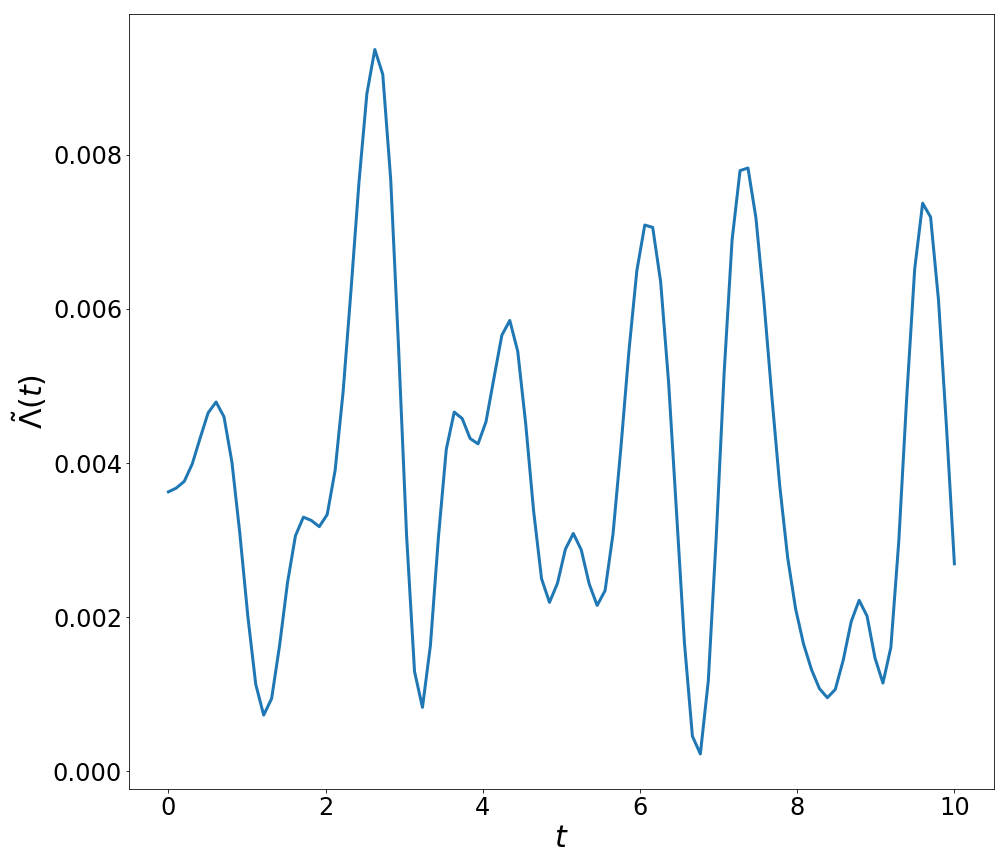
\includegraphics[scale=0.18]{figures/axialInteractingQuenchMassless.png}
	\end{minipage}%
	\begin{minipage}{0.5\textwidth}
		\centering(B)
		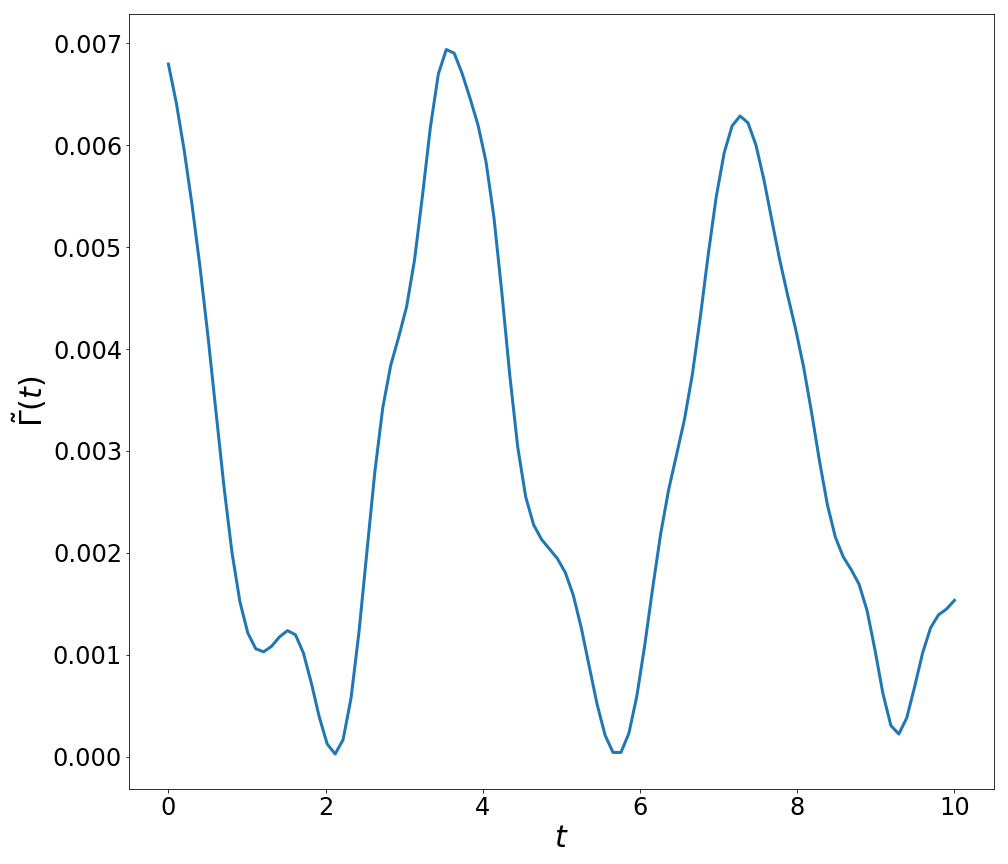
\includegraphics[scale=0.18]{figures/chiralInteractingQuenchMassless.png}
	\end{minipage}
	\caption{Plot of the order parameters as a function of time  for a quantum quench between the massless interacting Hamiltonian with $\mathcal{E}_0=0.0$ to the massless interacting Hamiltonian with $\mathcal{E}_0=0.5$. (A) Axial fermion density. (B) Density of chiral condensate.}\label{fig:orderparamsquech}
\end{figure}

\section{Comments and conclusion}

Throughout this chapter, we have numerically studied the lattice Schwinger model in all of its variants, i.e. the free massless Schwinger model, the free massive Schwinger model and the massless \& massive interacting model with and without a background electric field. We have used the exact diagonalization methods in order to simulate and study lattice models with a small number of degrees of freedom. To this end, we employed the python package \textit{Quspin}, to facilitate the numerical computations. For the free massless model, we computed its spectrum in real space and the single particle spectrum and commented on the structure of the half-filled band. Moreover, we showed, by simulating systems with increasing size, that the vacuum energy density in the limit of an infinite number of lattice sites tends to the value $-1/\pi$. This value is the continuum limit energy density for the XX-model which we showed was equivalent to the free Schwinger model. For the free massive model, we also studied the spectrum for varying mass and commented on the appearance of distinct eigenvalue manifolds as a consequence of the degeneracy of the eigenstates of the mass Hamiltonian. We computed the ground state and the first excited states energy densities and commented on the appearance of a spectrum energy gap due to the mass term. And furthermore, we confirmed that the energy gap should be linear with mass.\\

With respect to the interacting model, we computed its ground state energy density and showed it reduces to the case of the free model whenever the mass is zero. Additionally, we computed the values of the axial fermion and chiral condensate order parameters for various values of the background field. We observed that the value $\mathcal{E}_0=0.5$ is special since it separates the possible values of the order parameters in two distinct values at strong coupling. And we commented qualitatively how from the overall form of the chiral condensate density order parameter one can suspect the appearance of a critical behavior.\\

Finally, in the last section, we briefly introduced quantum quenches and described their importance. Subsequently, we studied global quenches starting from the free Hamiltonian to the interacting Hamiltonian with zero and non-zero background field. We computed the Loschmidt echo density and the expectation value of the chiral condensate density parameter and briefly commented of their dynamics. Also, we simulated a different global quench this time going from the interacting model with zero background field to the interacting model with non-zero background field. In this context, we studied the Loschmidt echo density and the dynamics of the axial fermion density and chiral condensate density parameters which were interesting since we know from chapter one the model shows critical behavior whenever $\mathcal{E}_0=0.5$. All three of this quantities showed oscillatory behaviors that we trace back to the dynamics of pair production due to the background electric field.


